\subsection{Minimum Return difference LQR/LQG}
Der offene LQR-Regelkreis 
\begin{equation*}
    L_{\textnormal{LQR}} = K\cdot \big(s\cdot I - A\big)^{-1}
\end{equation*}
besitzt hervorragende Robustheitseigenschaften:
\begin{equation*}
    \mu_{\textnormal{min,\textbf{LQR}}} = \min_\omega\bigg( \min_i\sigma_i\Big(I + L_{\textnormal{\textbf{LQR}}}(\jw)\Big)\bigg) \geq 1
\end{equation*}
Jedoch kann keine Aussage zur minimum return difference des LQG-Reglers gemacht werden.
\begin{equation*}
    \mu_{\textnormal{min,\textbf{LQG}}} = \min_\omega\bigg( \min_i\sigma_i\Big(I + L_{\textnormal{\textbf{LQG}}}(\jw)\Big)\bigg) \geq \ ?
\end{equation*}
Man muss nach der Reglerauslegung deshalb zwingend die Robustheit des Reglers überprüfen.

\subsection{Loop-Transfer Recovery LTR}
    Man kann die Robustheit des ursprünglichen LQR-Reglers mit einem LQG Regler approximieren. Dafür muss der Observer sehr schnell gewählt werden. Dadurch konvergiert der Fehler $e(t) = x(t)- \widehat{x}(t)$ schnell zu Null (im Grenzfall unendlich schnell). Diese Wiederherstellung der Robustheit nennt man \textit{loop-transfer recovery (LTR)}.
    
    \textbf{Erinnerung:} Je kleiner man den tuning-Parameter $q$ wählt, desto schneller wird die Dynamik des Fehlers (Schneller $\widehat{=} \ \operatorname{eig}\big(A - L(q)\cdot C\big)$ sind weiter links in der kommplexen Ebene)
    
    \subsubsection{Dynamik des Fehlers in der Zustandsschätzung}
        Analyse des Fehlers für $\displaystyle\lim_{q\to0}(\cdot)$.
        \begin{equation*}
            \lim_{q\to0}e(t) = \lim_{q\to0}\big(A - L(q)\cdot C\big)^{-1}\cdot\Dot{e}(t) = 0
        \end{equation*}
        Da $\big(A - L(q)\cdot C\big)$ Hurwitz ist und $\operatorname{eig}(X^{-1}) = 1/\operatorname{eig}(X)$ gilt,  konvergieren die Eigenwerte von $\big(A - L(q)\cdot C\big)$ asymptotisch gegen null. Mit $e(t) = x(t) - \widehat{x}(t)$ folgt:
        \begin{equation*}
            \lim_{q\to0} \widehat{x}(t) = x(t), \quad \forall t
        \end{equation*}
        
        Das System verhält sich für kleine $q$ als ob keine Beobachterdynamik vorhanden wäre. Für $q\to 0$ Verhält sich ein LQG-Regler wie ein LQR-Regler und besitzt somit die gleichen Robustheitseigenschaften.
        
        \textbf{Bemerkungen:}
        \begin{itemize}
            \item $q$ kann in der Realität nicht beliebig klein gewählt werden, da ansonst hochfrequentes Rauschen massiv Verstärkt wird.
            
            \item Falls die Regelstrecke nicht-miniphasige NST hat, approximiert der LTR-Ansatz den LQR-Regler häufig so gut wie möglich. (Bei nicht-miniphasigen Systemen. ist die durchtrittsfrequenz nah oben beschränkt und dadurch ist eine perfekte Approximation der LQR-Regelung nicht möglich.)
        \end{itemize}
        
        \begin{figure}[H]
            \centering
            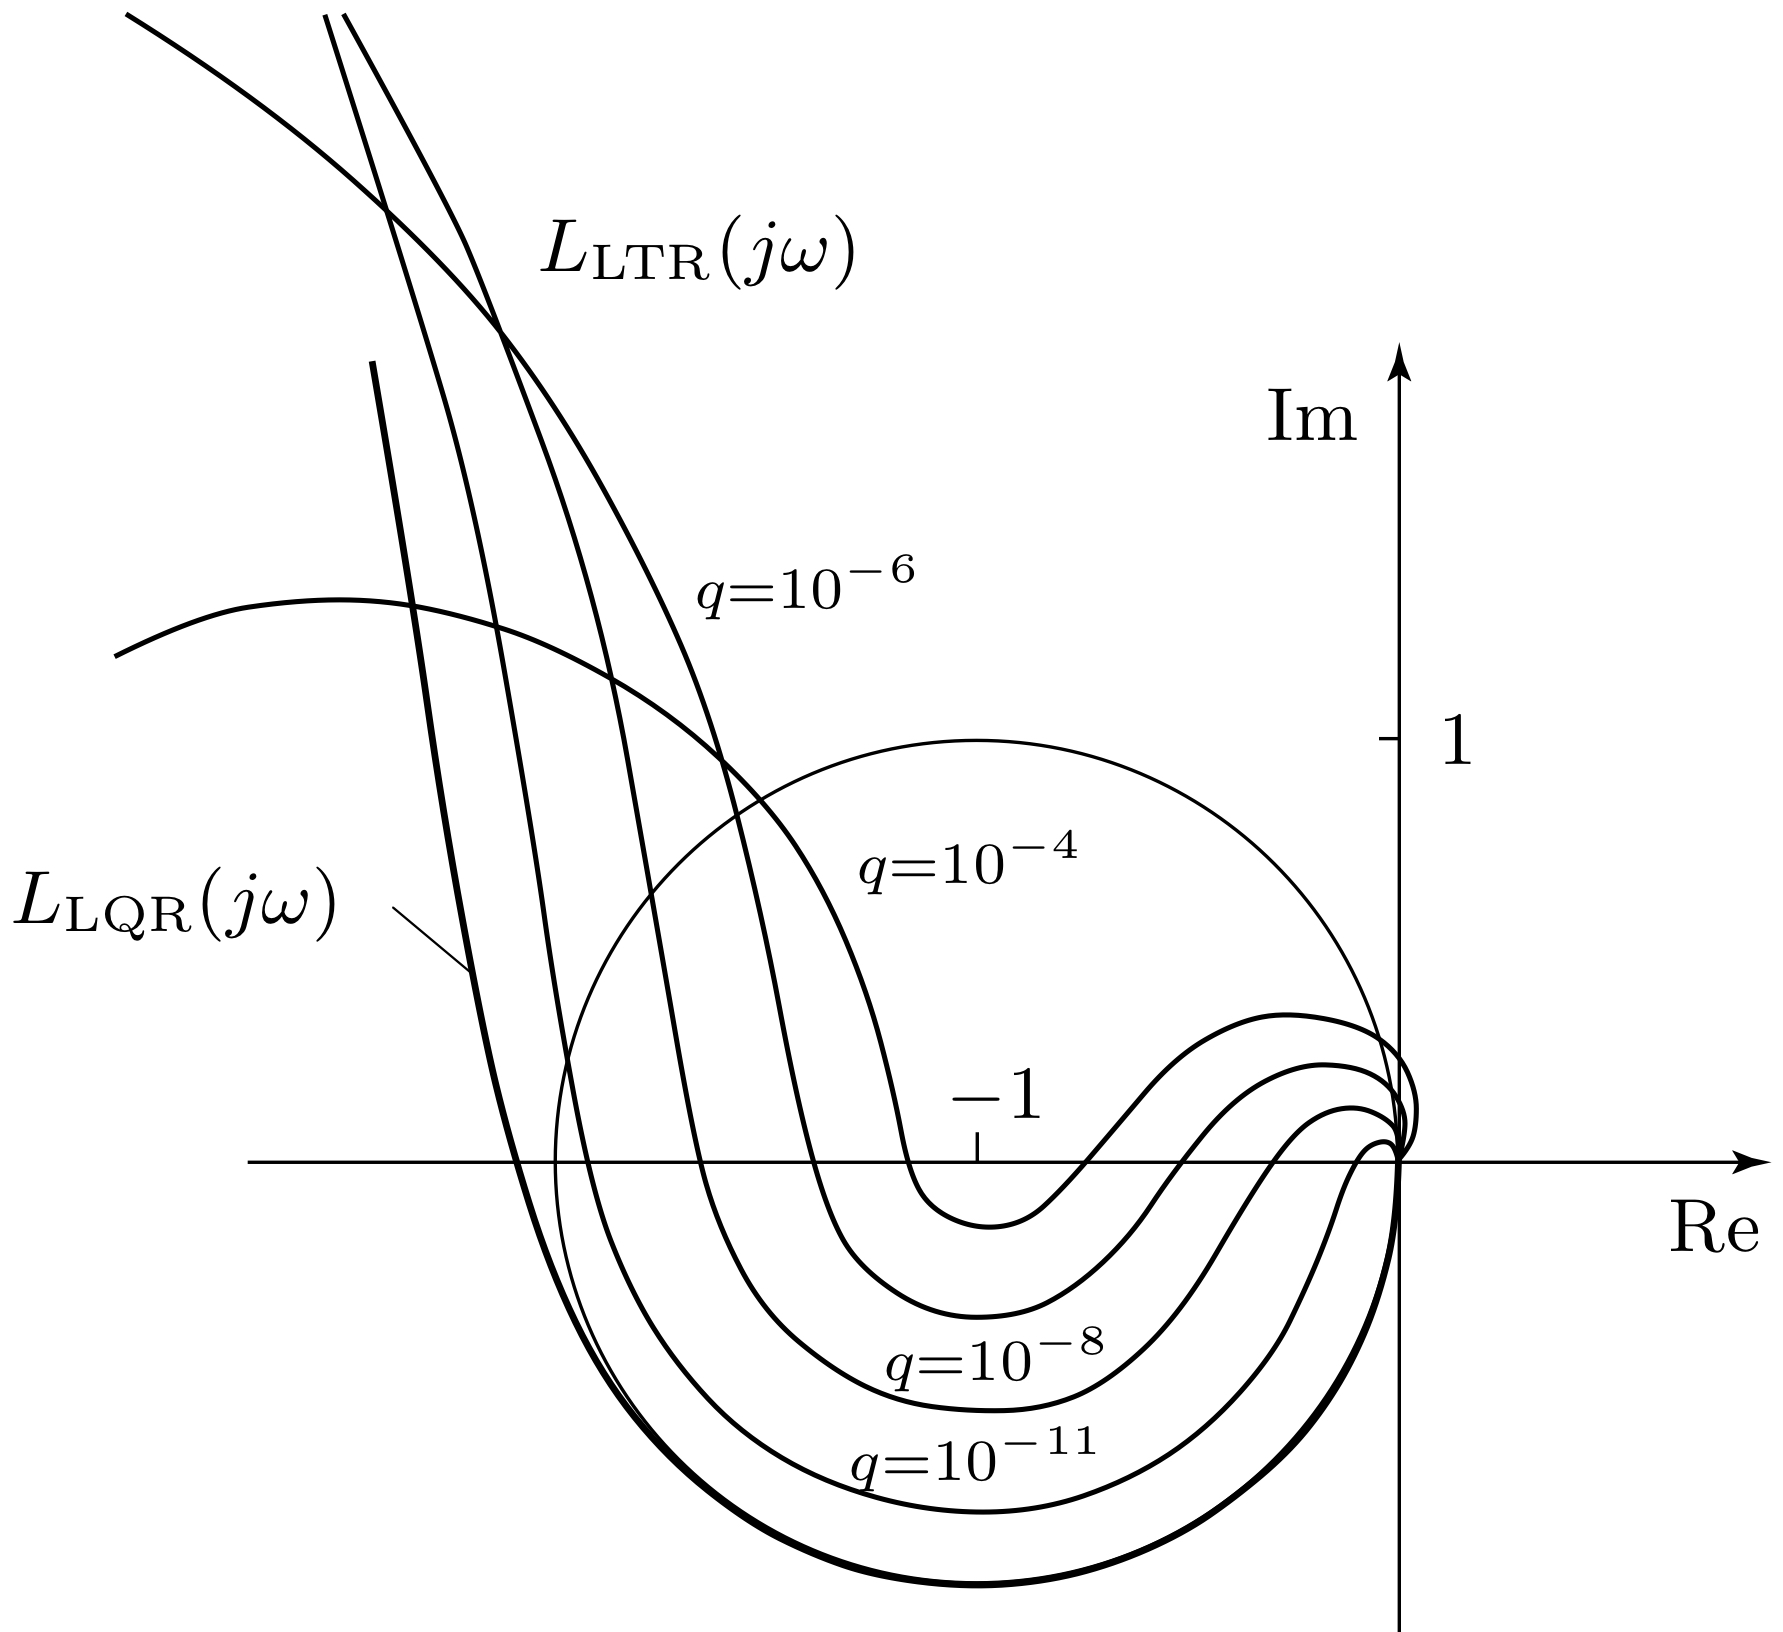
\includegraphics[width = 0.6\linewidth]{images/11/L_LTR.jpeg}
            \caption{$L_{\textnormal{LTR}}$ für verschiedene $q$.}
        \end{figure}
        